\section{Multimédia a jejich parametry, barevné modely, vzorkování, základní formáty obrazu, vlastnosti obrazu (statistická a psychovizuální redundance).}

\subsection{Multimédia a jejich parametry}

Multimédia je spojení dvou a více médií, mezi něž patří zvuk, obraz, video, text, animace apod. \textbf{Komprese} je proces, který odstraní z multimediálních dat redundantní a irelevantní složky za účelem snížení velikosti dat. \textbf{Parametry:} \textit{Barevný model}, \textit{Bitová hloubka obrazu} (maximální hodnota jasu udává schopnost dané reprezentace obrazu rozlišit různé úrovně jasu 8 bpp=$2^8$=256 odstínů), \textit{Jas} (svítivost pixelu 0--255 b), \textit{Poměr stran} (dán formátem obrazu nebo videa), \textit{Rozlišení obrazu} (udává šířku a výšku obrazu -- Mpx), \textit{Kontrast} (kvantifikuje rozdíl nebo podíl jasu mezi nejsvětlejšími a nejtmavšími oblastmi), \textit{Dynamický rozsah} (poměr mezi nejmenší a největší hodnotou jasu v obrazu), \textit{Snímková frekvence} (video, počet snímků/čas, 25 nebo 30 s/s pohyb je přirozený při použití prokládání, používá se ve standardním televizním vysílání), \textit{Prokládání} (video, bylo zavedeno z důvodu plynulosti pohybu ve videu při snímkových frekvencích 25 nebo 30 snímků za sekundu).

\subsection{Barevné modely}

Popisují barvy. Při kompresích se využívají zejména modely RGB, YUV, YCbCr.

\textbf{RGB} se používá  ve všech zobrazovacích jednotkách (televize, LCD displeje) a při snímání obrazu. Každá barva je lineární kombinace třech základních barev modelu. Lidský zrakový systém je nejvíce citlivý pravě na tyto složky (RGB). Variantou modelu RGB je model ARGB, kde je ke třem základním barvám přidán tzv. \textit{alfa kanál} označující průhlednost snímku.

\textbf{YUV} je používán ve standardních analogových video formátech PAL. Černobílé systémy
využívají pouze jasovou složku Y, barevné systémy využívají jak jasovou složku Y, tak i barvonosné složky U, V.

Barevný model \textbf{YCbCr} je používán v kompresních standardech JPEG, MPEG. Vychází z modelu YUV. Využívá se převodních vztahů z RGB. Y je jasová složka, Cb a Cr jsou chrominanční složky. 

\subsection{Vzorkování}

Lidské oko není citlivé na chrominanční složky stejně jako na jasové. Proto jsou tyto složky často podvzorkovávány. \textit{Model 4:4:4} -- matice Y,Cb a Cr mají shodnou velikost. \textit{Model 4:2:2} zachová jasovou složku v původním formátu, podvzorkuje horizontální rozlišení barvonosných složek na polovinu. \textit{Model 4:2:0} -- Cb a Cr matice – poloviční horizontální i vertikální rozlišení.

\subsection{Základní formáty obrazu}

HD (WXGA) (High Definition) 1280x720, FHD (Full High Definition) 1920x1080, WQHD (Wide Quad High Definition) 2560x1440, 4K UHD (4K Ultra-high-definition) 3840x2160.


\subsection{Vlastnosti obrazu (redudance)}

Méně důležité informace mohou být odstraněny v případě, že nedojde k narušení subjektivního vjemu lidského oka. Redundance může být rozdělena do dvou kategorií: 1. statistická redundance; 2. psychovisuální redundance.

Ke \textbf{statistické redundanci} patří redundance mezi pixely (prostorová redundance) a redundance kódová. \textbf{Prostorová redundance} je redundance uvnitř snímku. Autokorelace řádků (posunutých o jeden pixel) se blíží 1. Pro snížení redundance lze použít prediktivní kódování. Výstupem prediktivního kódování je potom rozdíl mezi aktuální a predikovanou hodnotou. Pro redukci redundance v čase se používají metody odhadu a kompenzace pohybu. \textbf{Kódová redundance} -- méně zastoupené symboly jsou kódovány větším počtem bitů. Využití kódování proměnné délky -- Huffmanovy kódy, slovníkové kódy a aritmetické kódy.

\textbf{Psychovisuální redundance} vyhází z lidského zrakového systému HVS (Human Visual System) -- citlivý na jasové detaily než na barevné detaily, citlivý na nízké frekvence než na vysoké, citlivý na velké kontrasty. \textit{Jasové maskování} (v případě, že rozdíl jasu jednotlivých objektů je velký, lidské oko objekty bez větších problémů rozezná), \textit{Prostorové maskování} (založeno na faktu, že vady obrazu, mezi něž patří například šum, jsou více viditelné na spojitých plochách), \textit{Frekvenční maskování} (oko je méně citlivé na vysoké frekvence -> potlačit), \textit{Dočasné maskování} (u video-sekvencí, kdy při změně scény ve videu lidské oko určitou dobu plně nevnímá detaily), \textit{Maskování barev }(více citlivý na jas než na barvu).

\section{Predikční kódování a skalární kvantizace (lineární, nelineární), vektorová kvantizace.}


\subsection{Predikční (prediktivní) kódování}

Existuje \textbf{vysoká korelace mezi sousedními pixely}. Filozofie prediktivního kódování je odstranění redundance mezi sousedními pixely a kódování pouze nové informace. Pixel je kódovaný jako \textbf{rozdíl mezi aktuální hodnotou a hodnotou predikovanou}, která je vypočítána z předchozí dekódované hodnoty. Prostorová redundance se vyskytuje mezi pixely v jednom snímku, zvláště pak sousední pixely jsou vysoce korelované. Pro potlačení vzájemné korelace se často používá diferenčního kódování DPCM.

%\vspace{-2cm}
\begin{figure}[ht]   
    \centering
    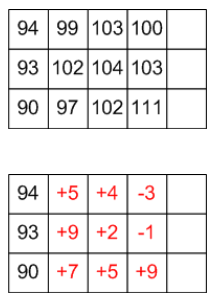
\includegraphics[width=0.22\linewidth]{images/image.png} 
\end{figure}
%\FloatBarrier 

\begin{enumerate}
    \item \textbf{Jedno-dimenzionální} -- k predikci využívají předešlý pixel na stejném řádku.
    \item \textbf{Dvou-dimenzionální} -- využívají pixelů v předchozích řádcích a pixelů ve stejném řádku.
    \item \textbf{Mezi-snímková} -- mohou využít jedno nebo dvou dimenzionální predikci, ale také pixely s předchozího kódovaného snímku.
\end{enumerate}

\subsection{Skalární kvantizace (lineární, nelineární)}

Hlavní mechanizmus pro ztrátu informace v kodérech obrazu a videa. Kvantizace využívá redundance podle HVS (Human Visual System). Při vhodně nastavené kvantizaci je těžké rozeznat degradaci obrazu. Nejjednodušší skalární kvantizátor je \textbf{lineární (uniformní) kvantizátor} u nějž je kvantizační krok konstantní. \textbf{Lineární (neuniformní) kvantizace} se vyznačuje tím, že velikost kvantizačních kroků je v celém intervalu různá (vyšší hustota v oblastech častějších hodnot signálu). Tento typ kvantizací se používá zejména u kompresí zvuku, u komprese obrazu se nevyužívá.


\subsection{Vektorová kvantizace}

Kódují se \textbf{vektory} (bloky), ne jednotlivé hodnoty jako u skalární kvantizace, je tedy efektivnější. Každý blok je kvantován určitým stupněm \textit{L}. \textit{L} kvantizačních stupňů = kódová kniha. Každý prvek kódové knihy obsahuje \textit{n} skalárních hodnot. Kódová kniha musí být známa v kodéru i dekodéru. Binární index nejbližšího vektoru kódové knihy je brán
jako výstup vektorového kvantizéru (\textbf{Voronoiův diagram}). (kódovou knihu o velikosti L = 3 a n = 2 -> V0 = [3,7], V1=[8,8], V2= [6,2]. Vstup [4,0] je kodován V0.) Příklad užití vektorová kvantizace barev v GIF (z původních 24 bitů na jeden pixel dostaneme po vektorové kvantizaci 4 bity na jeden pixel)

Komprese je dosažena použitím kódové knihy s relativně malým počtem vektorů oproti celkovému počtu obrazových vektorů. Kódová kniha je typicky vytvářená pomocí trénovací množiny obrazů zastupující obrazy, které mají být kódovány. K vytváření kódové knihy se může použít algoritmus LBG.

\begin{enumerate}
    \item Počáteční nastavení -- Množina trénovacích vektorů a zvolena kodová kniha R
    \item Nalezení změn pomocí trénovací množiny a předchozí kódové knihy -- Kódování trénovací množiny probíhá zařazením vektorů trénovací množiny do seskupení v okolí vektoru R; Výpočet výsledné průměrné MSE 
    \item Přizpůsobení množiny kódových slov za účelem snížení MSE -- Vypočítáme nové pozice vektorů v kódové knize

\end{enumerate}

\begin{figure}[ht]
    \centering
    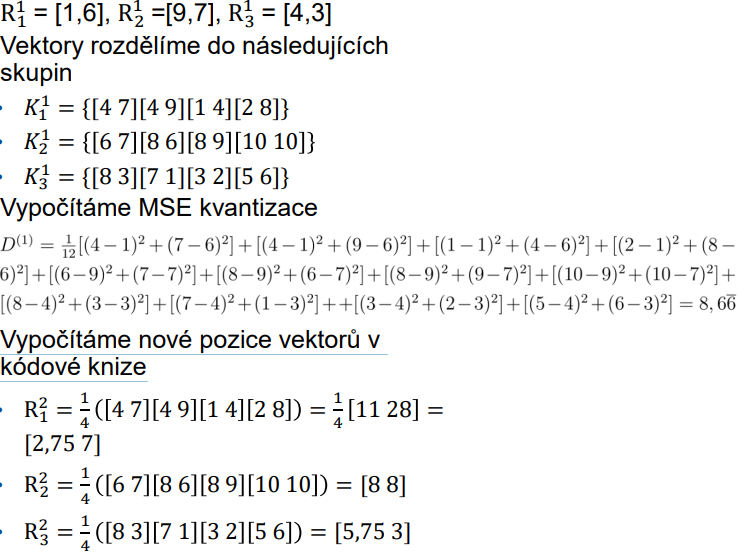
\includegraphics[width=0.5\linewidth]{images/LBG.png}
\end{figure}
\FloatBarrier


\section{Užívané metody pro odhad a kompenzaci pohybu u videu a jejich principy (FULL SEARCH, THREE STEP SEARCH, LOGARITMIC SEARCH), subpixelová přesnost při vyhledávání.}

Pro odhad a kompenzaci pohybu ve videu se nejčastěji používají \textbf{blokové metody}, které hledají nejlepší \textbf{shodu mezi bloky v po sobě jdoucích snímcích}. Základní princip je rozdělit snímek na bloky (8x8, 16x16) a pro každý blok v aktuálním snímku najít nejpodobnější blok v referenčním snímku v definovaném okolí (search window). Výsledkem je vektor pohybu pro každý blok, který popisuje jeho posun mezi snímky. 

Lidské oko nepostřehne rychlý pohyb objektů v plném rozlišení. Uprostřed prohledávací oblasti jsou porovnávány všechny pozice. Dále od středu je porovnávána pouze část možných bloků. Princip výběru lokality spočívá v tom, že dobrý výběr může být nalezen v okolí jiného dobrého výběru. V prvním kroku se v obraze hrubě stanoví podmnožina prohledávacích oblastí, v okolí nejpodobnějšího bloku se poté okolí prohledá dokonaleji.


\subsection{FULL SEARCH}

Je porovnáván každý možný blok v prohledávacím okně. Pro každou pozici se vypočítá míra podobnosti a vybere se ta s nejmenší chybou. Technika je výpočetně náročná (nevhodná pro reálný čas), ale přesná. Jiné nezkoumají se všechny možné bloky, hledají se spíše pouze lokální minima než globální.

\subsection{THREE STEP SEARCH}

Algoritmus vyhledává nejlepší blok ve třech krocích (případně \textit{N}). Vyhledávací
okno má danou velikost $S=2^{N}-1=4$ od středu oblasti.

\begin{enumerate}
    \item Nalezení pozice (0,0)
    \item Nastavení velikost kroku $S=2^{N-1}$
    \item Nalezení osmi pozic $+-4$ pixelů okolo pozice (0,0).
    \item Výběr pozice ze současných devíti s nejmenší chybou (\textit{MAE/SAE})
    \item Nastavení $S=S/2=2$
    \item Opakování bodů 3-5 do té doby, dokud $S\geq1$    
\end{enumerate}

\begin{figure}[ht]
    \centering
    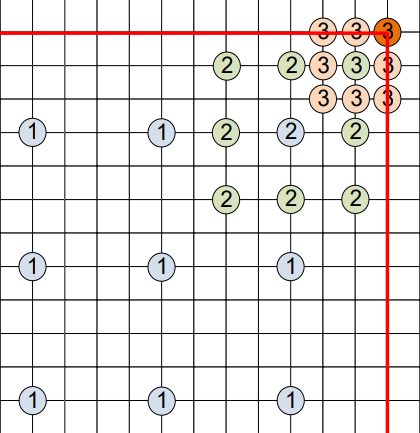
\includegraphics[width=0.3\linewidth]{images/tree.png}
\end{figure}
\FloatBarrier

\subsection{LOGARITMIC SEARCH}

Využívá logaritmické zmenšování kroku. V každém kroku se porovnává pět pozic. Pokud je nejlepší shoda ve středu, krok se zmenší na polovinu; jinak se střed posune na nejlepší pozici a krok zůstává stejný. Proces se opakuje, dokud krok není 1 pixel. Ještě méně výpočtů než \textit{TSS}, rychlé konvergování k optimu.

\begin{enumerate}
    \item Nalezení středové pozice (0,0), nastavení počátečního kroku $S$
    \item Nalezení čtyř pozic v horizontálním a vertikálním směru, $S$ pixelů od středové pozice. Pět pozic vytvoří tvar $+$
    \item Nastavení nového středového bodu do nejlepší pozice. Jestliže je nejlepším bodem bod středový, pak $S=S/2$, jinak $S$ zůstává nezměněné.
    \item Jestliže $S=1$, přechází se k bodu 5, jinak do bodu 2.
    \item Vyhledání osmi pozic v okolí poslední středové pozice. Nalezení bloku s nejmenší chybou z devíti prohledávaných.
\end{enumerate}

\begin{figure}[ht]
    \centering
    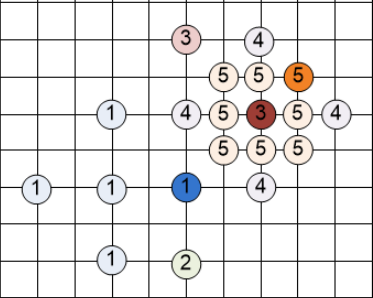
\includegraphics[width=0.3\linewidth]{images/TSS.png}
\end{figure}
\FloatBarrier

\subsection{Subpixelová přesnost při vyhledávání}

Subpixelová přesnost při vyhledávání znamená, že pozice nebo vektor pohybu nejsou určovány jen s přesností na celý pixel, ale i na jeho zlomky. To umožňuje výrazně zpřesnit výsledky, protože skutečný pohyb objektů mezi snímky (v interpolované oblasti) často neodpovídá přesně celočíselným posunům.

\begin{itemize}
    \item Horizontální interpolace -- h = (A + B) / 2
    \item Vertikální interpolace -- v = (A + C) / 2
    \item Centrální interpolace -- c = (A + B + C + D) / 4
\end{itemize}


\section{Entropické kódování (aritmetické, LZW, Huffmanovo) princip a jejich využití při kompresi obrazu a videa.}

\begin{itemize}
    \item Huffmanovo kódování -- komprese obrazů JPEG, komprese videí MPEG, H.26x
    \item Aritmetické kódování -- komprese obrazů JPEG, komprese videí MPEG, H.26x
    \item Slovníkové metody kódování -- komprese obrazů GIF, PNG
\end{itemize}

\subsection{Huffmanovo kódování}

Patří do tzv. prefixových kódů. \textbf{Více se vyskytující symboly jsou kódovány menším počtem bitů}, naopak méně se vyskytující symboly jsou kódovány větším počtem bitů. Výsledkem je snížení průměrného počtu bitů na jeden symbol. Huffmanovy kódy mají pouze \textbf{délku celých bitů}. Vysoké psp kódovaný více než je nutné (P=0,9, opt. délka I=-log2(0,9)=0,15, ale délka kódů bude 1 bit.)

\begin{figure}[ht]
    \centering
    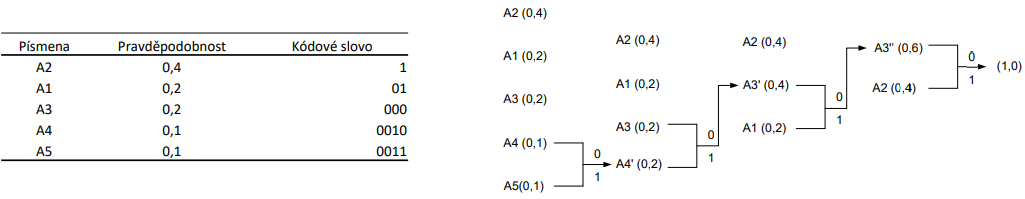
\includegraphics[width=0.9\linewidth]{images/huff.png}
\end{figure}
\FloatBarrier


\subsection{Aritmetické kódování}

Aritmetické kódování na rozdíl od Huffmanova nekóduje jednotlivé symboly,
ale \textbf{celé zprávy} nebo jejich části (Eliminace problému s přesností na jeden bit). Výstupem kódování je číslo spadající do intervalu <0,1). 

\begin{figure}[ht]
    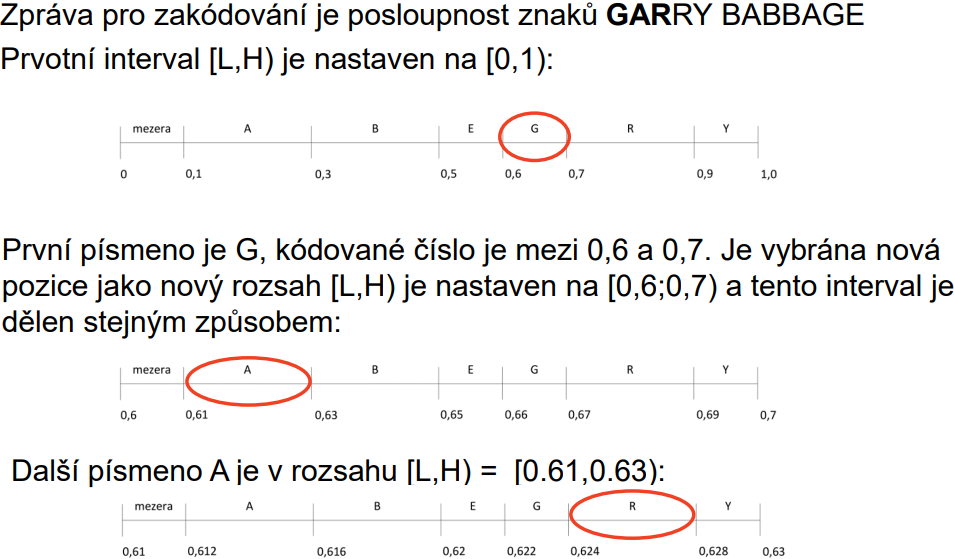
\includegraphics[width=0.7\textwidth]{images/ar.png}
    \hfill
    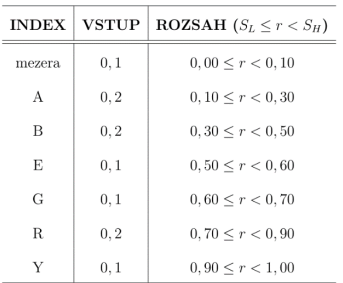
\includegraphics[width=0.3\textwidth]{images/hufff.png}
\end{figure}
\FloatBarrier

\subsection{LZW}

Slovníkové metody kódování využívající \textbf{dynamický slovník} z pohledu LZ2. Vstupy kódovány pouze do  <i>: i -- index položky slovníku. Slovník obsahuje všechna
písmena zdroje – musí být znám v kodéru i dekodéru. Poslední písmeno každého výrazu je zároveň první písmeno výrazu následujícího.

\begin{figure}[ht]
    \centering
    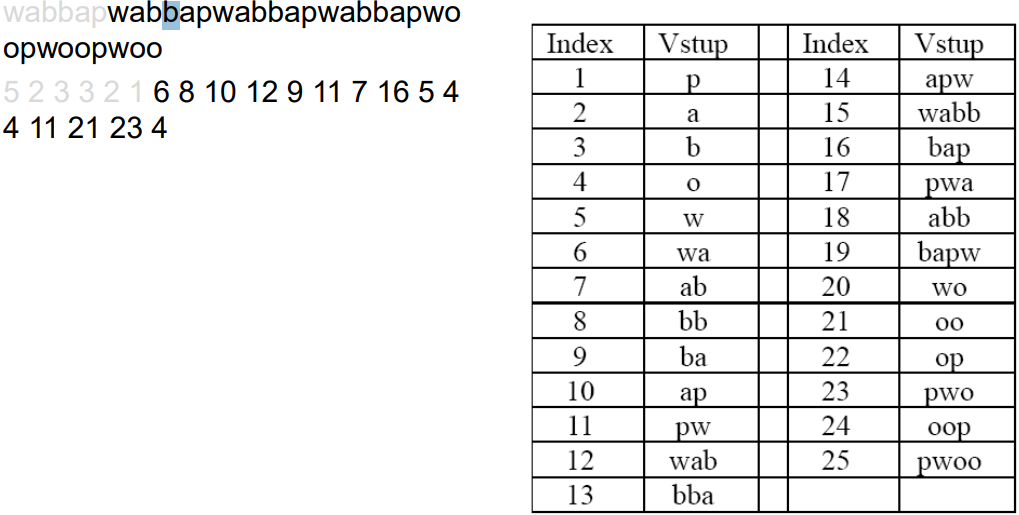
\includegraphics[width=0.7\linewidth]{images/LZW.png}
\end{figure}
\FloatBarrier


\section{Transformace obrazových dat (DCT, DWT, WHT) - základní princip a jejich využití při kompresích obrazu a videa.}


Vzorky z prostorové oblasti jsou transformovány do jiné reprezentace. Transformační kódování se zaměřuje na korelaci mezi pixely. Transformační kódování \textbf{koncentruje energii do malého počtu vzorků}, které jsou však velmi důležité -- dekoreluje vstupní data.

\subsection{DCT -- Diskrétní kosinová transformace}

Většinou aplikována na malé bloky 8x8 (JPEG, H.261, H.263, H.263+, MPEG-2, MPEG-4). Frekvence v 2D transformační kosinové matici vzrůstá od levého horního rohu k pravému spodnímu rohu diagonálním směrem. První koeficient $c1$ bude mít vysokou hodnotu, ostatní by měly mít nízkou hodnotu. Pokud jsou vstupní data hodně korelována, velký počet DCT koeficientů je roven 0.

Transformační matice libovolné velikosti $N*N$ se odvozuje podle vztahů. 2D transformace maticově -- dopředná transformace má tvar $\boldsymbol{C=WDW^T}$, zpětná transformace má tvar $\boldsymbol{D=W^TCW}$, kde $C$ je transformovaná matice, $W$ je transformační matice a $D$ je vstupní matice.


\subsection{DWT -- Diskrétní vlnková transformace}

Aplikována na větší bloky (tiles) nebo na celý obraz (JPEG 2000, MPEG-4). Pro praktickou ukázku vlnkové transformace byla vybrána jednoduchá vlnka – Haarova
vlnka, po níž se jmenuje i transformace.

\begin{figure}[ht]
    \centering
    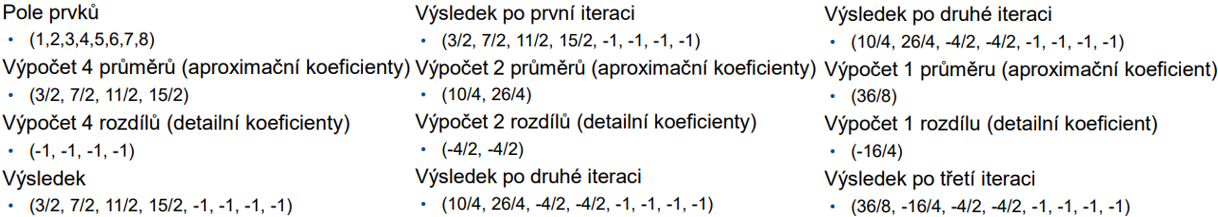
\includegraphics[width=1\linewidth]{images/dwt2.png}
\end{figure}
\FloatBarrier

\begin{figure}[ht]
    \centering
    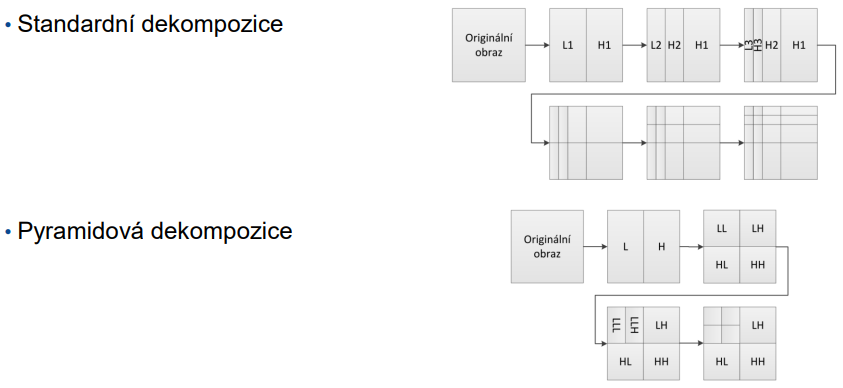
\includegraphics[width=0.7\linewidth]{images/dwt.png}
\end{figure}
\FloatBarrier

\subsection{DWHT -- Diskrétní Walsh-Hadamard Transform}

Celočíselná transformace aplikovaná v kodeku H.264, H.265. Diskrétní Walsh-Hadamardova transformace (DWHT) je oproti kosinové velmi jednoduchá, rychlá a celočíselná. Transformační matice je vytvořena z diskrétní Hadamardovy matice $H$ o velikosti $N*N$, rozměry jsou vždy mocninou dvou ($2^N$). $H_{2^N}=\bigl(\begin{smallmatrix}
H_{N} & H_{N} \\
H_{N} & -H_{N} \\
\end{smallmatrix}\bigr)$.

\begin{figure}[ht]
    \centering
    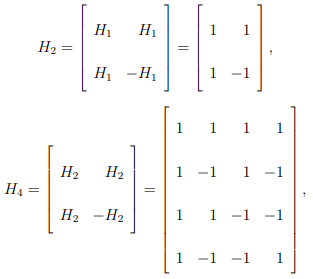
\includegraphics[width=0.3\linewidth]{images/wht.png}
\end{figure}
\FloatBarrier

Transformační matice pro DWHT se získá normalizací Hadamardových matic koeficientem $\frac{1}{\sqrt{N}}$.

\section{K čemu slouží metody SPIHT a EZW při kompresích obrazu či videa, popište jejich princip.}

Jedná se o entropické kódování koeficientů využívané při DWT. \textbf{Cíle kódován}í -- kódovat nejprve důležité informace a možnost kdykoliv ukončit kódování/dekódování, mít v době ukončení ty nejlepší možné výsledky.


\subsection{EZW}

Koeficienty vlnkové transformace jsou uspořádány do \textbf{stromové struktury}, kde \textbf{kořen} představuje \textbf{nízkofrekvenční} složky a potomci vyšší frekvence. Většina koeficientů je po transformaci blízká nule, což EZW využívá: pokud je koeficient i všichni jeho potomci menší než stanovený práh, označí se jako kořen nulového stromu (zerotree root) a kóduje se jediným symbolem. To výrazně snižuje množství potřebných dat pro popis nevýznamných oblastí obrazu.

Každý kořen má 4 potomky (1 u koeficientů v nejnižším subpásmu). Pokud má kořen malou velikost, všichni
jeho potomci mají malou velikost.

\begin{itemize}
\item \textbf{Významný koeficient kladný (SP -- Significant Positive)} --  koeficient, jehož velikost je větší než stanovený práh $T$.

\item \textbf{Významný koeficient záporný (SN -- Significant Negative)} -- koeficient, jehož velikost je větší než záporná hodnota stanoveného prahu $T$.

\item \textbf{Kořen nulového stromu (ZTR -- Zerotree Root)} -- koeficient, jehož velikost je menší než stanovený práh $T$ a všechny potomci jsou nevýznamní.

\item \textbf{Izolovaná nula (IZ -- Isolated Zero)} -- koeficient, jehož velikost je menší než stanovený práh $T$ a někteří potomci jsou významní.
\end{itemize}

\begin{enumerate}
    \item Inicializace -- Všechny koeficienty jsou nevýznamné, počáteční práh $T_o = 2^{\lfloor \log_2 c_{max} \rfloor}$
    \item V každém průchodu je práh snížen o polovinu T/2.
    \item Po průchodu je každý významný koeficient upřesněn +/-T/4.
\end{enumerate}

\begin{figure}[ht]
    \centering
    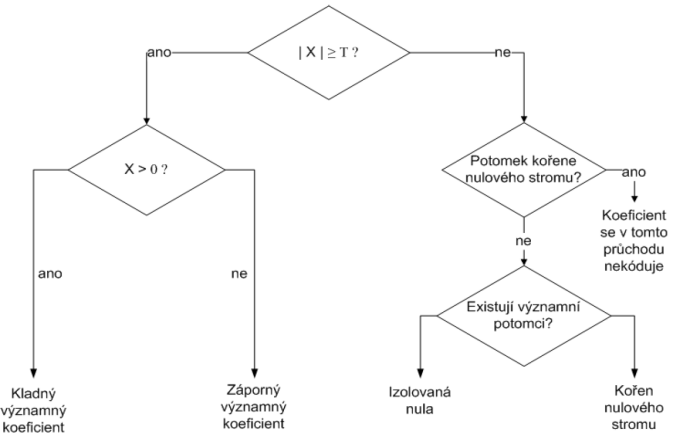
\includegraphics[width=0.6\linewidth]{images/ezw.png}
\end{figure}
\FloatBarrier


\subsection{SPIHT}

Rozdíly od EZW -- \textbf{přesnost} -- EZW: 4 symboly (SP, SN, ZTR, IZ) -> SPIHT: binární přesnost. \textbf{Vztahy mezi koeficienty} -> EZW: Každý koeficient aproximačního pásma s nižší frekvencí má 3 potomky, ostatní koeficienty mají vždy 4 potomky. -> SPIHT: Koeficient v levém horním rohu nemá potomka, ostatní koeficienty mají
vždy 4 potomky. Při kódování využívá dělení \textbf{stromů} tak, aby nevýznamné koeficienty zůstávaly v jedné větší množině.

Stromy používané ve SPIHT jsou děleny na čtyři typy množin. Tyto množiny patří
vždy k jednomu kořenu na pozici (\textit{i, j}):

\begin{figure}[ht]
    \centering
    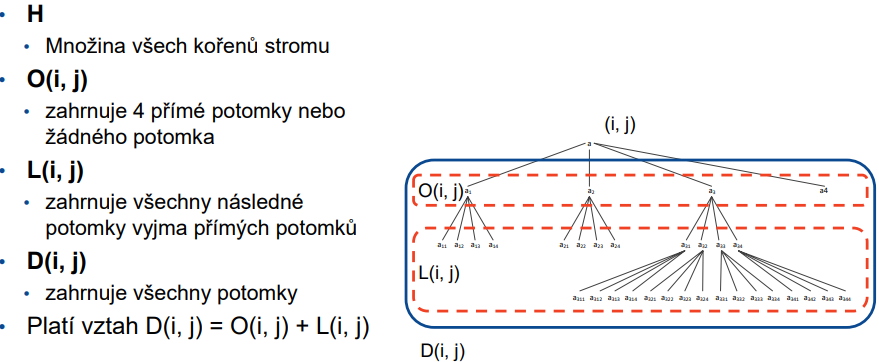
\includegraphics[width=0.7\linewidth]{images/spiht.png}
\end{figure}
\FloatBarrier

Algoritmus SPIHT využívá \textbf{tři typy seznamů}: \vspace{-4mm}
\begin{itemize}
    \item Seznam nedůležitých pixelů \textit{LIP} -- obsahuje pozice koeficientů.
    \item Seznam důležitých pixelů \textit{LSP} -- obsahuje pozice koeficientů.
    \item Seznam nedůležitých množin \textit{LIS} -- obsahuje pozice kořenů množin typu $D$ nebo $L$.
\end{itemize}

Zatím na to nemám síly -- DODĚLAT!!!!!!

\section{Zabezpečení obrazových dat vodoznačením – principy, techniky.}

Technika k ověření identity a autenticity vlastníka digitálního obsahu (obrazu, videa, audia). \textbf{Využití pro:} Ochranu autorských práv, Monitorování pohybu zdrojových dat (Každý příjemce dostane multimediální data s jiným vodoznakem. Pokud obsah předá dalšímu, pozná se, kdo jej zneužil), Anotaci digitálního obsahu. Vodoznačící techniky umožňují vložit vodoznak do originálních dat. Později může být vodoznak detekován a vyjmut.  Jedním z jeho nejdůležitějších parametrů je jeho odolnost. \textbf{Požadavky:}

\begin{enumerate}
\item \textbf{Nevnímatelnost} -- nepřesáhnout práh citlivosti zraku či sluchu člověka.
\item \textbf{Odolnost} -- bez znalosti použité metody a tajného klíče vodoznak nelze odstranit. Odolnost proti modifikacím dat.
\item \textbf{Bezpečnost} -- Použití kryptografických klíčů k zašifrování vkládaného vodoznaku.
\item \textbf{Složitost} -- Platí pravidlo, že prolomení vodoznaku by mělo trvat takový čas, aby po jeho úspěšném prolomení byla data bezvýznamná.
\item \textbf{Statická nedetekovatelnost} -- Nemělo by být možné z více dat zabezpečených stejným vodoznakem detekovat vodoznak.
\item \textbf{Kapacita} -- Množství informace, které může být uloženo do zdrojových dat.
\item \textbf{Spolehlivost detekce} -- Dostatečně spolehlivý k prokázání vlastnictví k danému dílu.
\end{enumerate}

Návrh zahrnuje výběr oblasti, kde bude informace zakryta. Volba domény pro vodoznačení (prostorová, transformační). Pseudonáhodný generátor čísel, udávající náhodnou pozici pixelů, které budou použity k vodoznačení. Inicializace tajným nebo veřejným klíčem.


\subsection{Prostorová oblast}

Menší výpočetní náročnost. Menší odolnost vůči útokům. Využívá se různých barevných prostorů, nejčastěji \textit{RGB}, \textit{YCbCr} (nejčastěji využívá složka \textit{Y} -- nebývá podvzorkována). Časté využití nejméně významných bitů LSB. Obrazy zabezpečené těmito technikami jsou však velmi \textbf{náchylné na jakýkoli útok}. Z toho důvodu nejsou pro zabezpečení autorských práv příliš vhodné.

Nejdůležitějším parametrem pro vložení vodoznaku je parametr hloubka
vložení \textit{h}. Ten definuje, jaká z bitových hladin originálního obrazu $C_{0}$ bude využita pro vložení permutovaného vodoznaku \textit{W}. Na základě parametru \textit{h} se tedy vynulují veškeré bity v dané hladině originálního obrazu \textit{Co}, čímž vznikne obraz \textit{Co*} připravený pro vložení vodoznaku. Z binárního permutovaného vodoznaku \textit{W} se vytvoří osmibitový vodoznak \textit{W*}, kde všechny hladiny, kromě hladiny \textit{h}, budou nulové. Hladina \textit{h} bude obsahovat hodnoty binárního vodoznaku. Vlastní vodoznačení poté probíhá prostým součtem obou upravených obrazů (\textit{Cw=Co*+W*}).

\begin{figure}[ht]
    \centering
    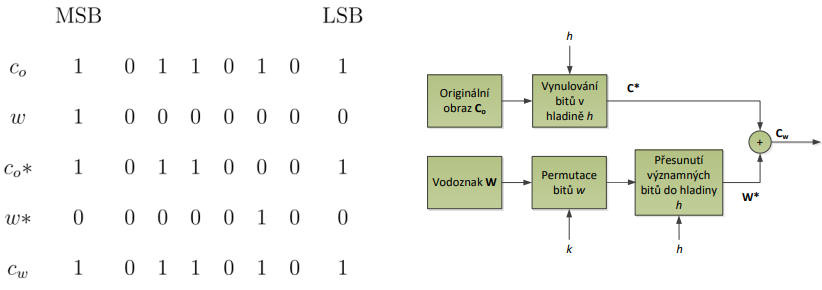
\includegraphics[width=0.75\linewidth]{images/fr.png}
\end{figure}
\FloatBarrier

\subsection{Frekvenční oblast}

Pro převod z prostorové do frekvenční oblasti se nejčastěji využívají 2D-DCT a 2D-DWT. Vodoznak je \textbf{vkládán} do originálních dat \textbf{pomocí dvou koeficientů ve frekvenční oblasti} vybraných bloků 8x8. Koeficienty jsou vybírány z oblasti \textbf{středních frekvencí}. Využívá se koeficientů, které jsou kvantovány \textbf{stejným} počtem kvantizačních hladin. Častěji se využívá vkládání do frekvenční oblasti \textbf{jasové složky \textit{Y}}.

Při vkládání vodoznaku do originálních dat se použijí koeficienty \textit{(u1, v1), (u2, v2)} ve frekvenční oblasti, kde \textit{ui} a \textit{vi} definují pozici bodů v transformovaném bloku frekvenčních koeficientů o rozměru 8x8 prvků. Tyto dva koeficienty jsou vybírány z oblasti středních frekvencí. Při vkládání vodoznaku jsou používány takové koeficienty \textit{u}, \textit{v}, které jsou kvantovány stejným počtem kvantizačních hladin. Z doporučené kvantizační tabulky pro jasové složky u komprese JPEG plyne, že vhodnými koeficienty jsou například (3,1) a (4,1), (4,3) a (5,2), (1,4) a (3,3) a další. Pro zvýšení odolnosti vloženého byl zaveden koeficient hloubky vložení \textit{h}.

Ve frekvenční oblasti je možné vodoznak vložit do libovolného frekvenčního pásma, avšak modifikacemi \textit{nízkofrekvenčních} složek dochází k degradaci výsledného obrazu. Na druhé straně při vložení vodoznaku do oblasti \textit{vysokofrekvenčních} složek dochází po většině útoků k odstranění vodoznaku. Doporučuje se vodoznak vkládat do oblasti \textit{středních} frekvencí.

\begin{figure}[ht]
    \centering
    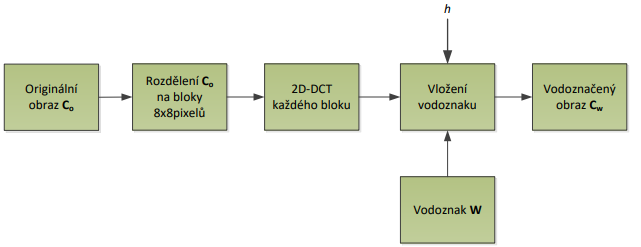
\includegraphics[width=0.65\linewidth]{images/ffff.png}
\end{figure}
\FloatBarrier

\section{Popište kompresi obrazu JPEG a PNG a definujte rozdíly.}

\subsection{JPEG -- Joint Picture Expert Group}
První mezinárodní standard pro kompresi barevných, šedotónových a černo-bílých
digitálních statických obrazů, *.jpg. Podporuje \textbf{ztrátovou} (založenou na diskrétní kosinové transformaci (DCT) i \textbf{bezeztrátovou}
(založenou prediktivním kódování) kompresi.

Komprese \textbf{není} závislá na: \vspace{-4mm}
\begin{enumerate}
    \item Prostorovém rozlišení obrazu
    \item Poměru stran obrazu
    \item Barevném modelu
\end{enumerate}

Celkem 4 módy kódování:  \vspace{-4mm}
\begin{enumerate}
    \item \textbf{Základní mód} –- ztrátové kódování (komp. poměr ~1:20), využívá DCT, Huffmanovo kódování
    \item \textbf{Rozšířený mód} –- ztrátové kódování, progresivní kódování, DC všech bloků, 1. AC všech bloků
    \item \textbf{Bezeztrátové kódování} -- prediktivní kódování, nevyužívá DCT
    \item \textbf{Hierarchické kódování} –- několik prostorových rozlišení
\end{enumerate}

\textbf{Postup:} \vspace{-4mm}
\begin{enumerate}
    \item Formát vstupu -- rozlišovací schopnost 8 bitů/pixel, standardně model RGB.
    \item Převedení z R\textbf{GB na YCbCr}
    \item \textbf{Podvzorkování} Cb a Cr složky (jasová složka je citlivější na oko než barevná) -- 4:2:2, 4:2:0
    \item Rozdělení na \textbf{8x8px bloky}
    \item \textbf{Provedení DCT} (Diskrétní kosinová transformace) -– potlačení korelačních vazeb mezi vzorky, koncentrace energie signálu do oblasti nízkých frekvencí, zanedbání vyšších frekvencí, zaokrouhlení frekvenčních kvocientů, není ztrátová.
    \item \textbf{Kvantizace} -– po DCT se energie soustředí k levému hornímu rohu (nízká frekvence), koeficienty představující vyšší frekvenci mají nízké hodnoty, při vynulování koeficientů s vyššími frekvencemi dochází pouze k nepatrné ztrátě kvality -- zavedení malé chyby do nízkých a velké do vysokých frekvencí, při kvantizaci dochází k zásadní \textbf{ztrátě informace}, kvantizační tabulky nejsou standardizované, jsou zvlášt pro jasovou a barevnou složku, kvalita výsledného obrazu je ovlivněna faktorem kvantizace.
    \item \textbf{Čtení zik-zak} -– od nejnižší po nejvyšší frekvenci, koeficienty DCT jsou čteny od nejnžší frekvence po nejvyšší.
    \item Provedení \textbf{Huffmanova (aritmetického) kódování} -- dle Huffmanových tabulek, v datovém toku jsou uloženy Huffmanovy i kvantizační tabulky.
\end{enumerate}

\begin{figure}[ht]
    \centering
    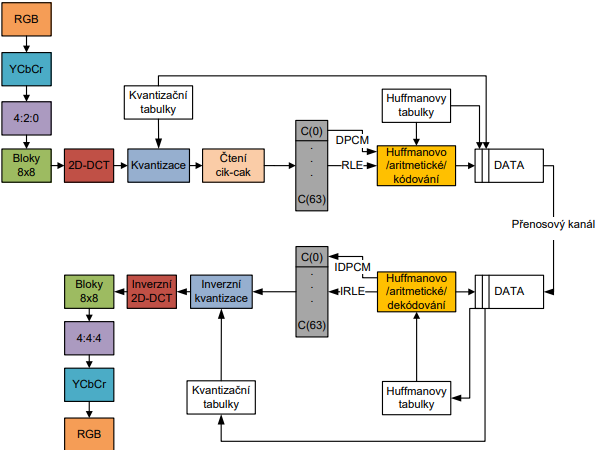
\includegraphics[width=0.65\linewidth]{images/jpeg.png}
\end{figure}
\FloatBarrier

\subsection{PNG}

Kompresní formát pro digitální obrazy s podporou jak ztrátové, tak i bezeztrátové komprese. Podpora 24 a 32 bitové barevné hloubky, podpora osmibitové průhlednost (tzv. alfa kanál).

\begin{enumerate}
    \item \textbf{Separace alfa kanálu} -- alfa kanál se může odstranit v případě, kdy všechny složky alfa kanálu mají maximální hodnotu. Typicky model RGBA (0 nebo 1; u RGBA 0-256 -- definuje se úroveň průhlednosti)
    \item \textbf{Indexování barev} -- používá se v případě, že počet barev v barevné paletě je menší nebo roven 256 (formát PNG-8). Definuje se barevná paleta. Každému pixelu v obraze je přiřazena barva z barevné palety.
    \item \textbf{Sloučení RGB} -- v případě, že jednotlivé barevné kanály mají stejnou bitovou hloubku a pro každý pixel jsou hodnoty barevných složek RGB shodné, pak je možné barevné kanály sloučit do jednoho kanálu ve stupních šedé.
    \item \textbf{Zhutnění alfa kanálu} -- pokud obraz obsahuje alfa kanál a existuje jedna barva RGB pro kterou platí, že všechny pixely nesoucí tuto barvu jsou průhledné, zatímco ostatní pixely jsou neprůhledné, je možné alfa kanál vynechat a zapsat pouze informaci o kombinaci RGB která je průhledná.
    \item \textbf{Změna bitové hloubky} -- pokud je referenční obraz v jiné bitové hloubce než určuje tabulka, volí se nejbližší vyšší bitová hloubka a původní hodnoty jsou lineárně přepočteny do nových hodnot.
    \item \textbf{Prokládání pixelů} -- 2 varianty
        \begin{itemize}
            \item Bez prokládání -- pixely jsou z obrazu vyčítány nejprve po řádcích zleva doprava, shora dolů.
            \item S prokládáním (metoda Adam7) -- pixely obrazu jsou vyčítány v sedmi průchodech a každý další jej zjemňuje.
        \end{itemize}
    \item \textbf{Filtrace} -- Formát PNG specifikuje celkem 5 různých filtrů. Na každý řádek redukovaného obrazu (po prokládání) je možné použít rozdílné filtry (doporučení použití pouze 1 filtru). Filtry pracují přímo s byty, nikoliv pixely obrázku.
        \begin{enumerate}
    \item \textbf{Filtr typu 0 (None)} -- Žádný filtr, byty jsou ze vstupu přesně zkopírovány na výstup a nedochází k žádné změně. 

    \item \textbf{Filtr typu 1 (Sub)} -- od aktuálního bytu odečítá byte nalevo od něj, tedy $x = x - a$. Při rekonstrukci obrazu se rozdíl nahradí součtem, tedy $x = x + a$.

    \item \textbf{Filtr typu 2 (Up)} -- od aktuálního bytu odečítá byte nad ním, tedy $x = x - b$. Při rekonstrukci obrazu se rozdíl nahradí součtem, tedy $x = x + b$.

    \item \textbf{Filtr typu 3 (Average)} -- kombinuje dva předchozí filtry a odečítá průměrnou hodnotu bytů nalevo a nad aktuálním bytem, tedy $x = x - \left\lfloor (a - b)/2 \right\rfloor$ a zaokrouhluje na celé číslo směrem dolů. Při rekonstrukci obrazu se rozdíl nahradí součtem, tedy $x = x + \left\lfloor (a - b)/2 \right\rfloor$.

    \item \textbf{Filtr typu 4 (Paethův)} -- nejsložitější, porovnává absolutní hodnoty získané dle rovnic. $p = a + b - c,$ $pa = |p - a|,$ $pb = |p - b|,$ $pc = |p - c|$. Z nich vybere nejnižší hodnotu. Ta je následně odečtena od původního bytu. Při rekonstrukci obrazu se rozdíl nahradí součtem. 
        \end{enumerate}

        \begin{figure}[ht]
            \centering
            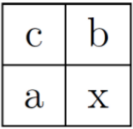
\includegraphics[width=0.1\linewidth]{images/filtr.png}
        \end{figure}
        \FloatBarrier

    \item \textbf{Komprese} -- Ke kompresi se používá algoritmus Deflate, pro dekompresi Inflate. Při kompresi se používá slovníkové kódování LZ77 společně s Huffmanovým kódováním. Komprese LZ77 hledá v komprimovaných blocích dat duplikovanou sérii bytů. Jakmile nějakou nalezne, je nahrazena značkou obsahující délku série a vzdáleností k předchozí shodě. Následuje \textbf{Huffmanovo kódování}, které dále snižuje počet bytů. Výsledný datový tok je uložen ve formátu \textit{zlib}.
\end{enumerate}

\subsection{Rozdíly}

\begin{table}[h]
\centering
\small
\begin{tabular}{|l|c|c|}
\hline
\textbf{Vlastnost}      & \textbf{JPEG}           & \textbf{PNG}           \\
\hline
Typ komprese            & ztrátová                & bezeztrátová           \\
\hline
Vhodné pro              & fotografie              & grafika, loga, text    \\
\hline
Kvalita po kompresi     & může se zhoršit         & beze změny             \\
\hline
Podpora průhlednosti    & ne                      & ano                    \\
\hline
Blokový artefakt               & může obsahovat          & nikdy                  \\
\hline
\end{tabular}
\end{table}



\section{Standardy pro kompresi videa MPEG a H.26x. Popište metody, které zvyšují účinnost komprese v moderních video standardech.}

\subsection{MPEG}
Umožňují ztrátovou kompresi videosekvence. Komprese pracuje jak s časovou, tak i s prostorovou redundancí. Je multimediální standard specifikující kódování obrazu a zvuku, standard na kompresi videa.

\subsubsection{MPEG-1}
\textbf{Navržen pro ukládání videa na CD}, formát vzorkování 4:2:0, 25 snímků/s, bitová rychlost 1-1,4 Mb/s

\textbf{Požadavky MPEG videa}: možnost zastavení obrazu, libovolný přístup ke snímkům obrazu v určitém čase (převíjení vpřed a vzad s přesností 0.5s), schopnost přehrávání vpřed i vzad s vyšší rychlostí než je normální rychlost videa, synchronizace audio a video stopy při přehrávání, práce v reálném čase

\begin{enumerate}
    \item \textbf{Přeuspořádání snímků} -- Přeskládání GOP – postup kódování je rozdílný od postupu přehrávání
    \item \textbf{Kódování 1. snímku v GOP} -- Snímek je transformován a kvantizován jako JPEG
\item Následně je kódován pomocí VLC (Variable length coding) a uložen do bufferu, před kódováním je zároveň zpětně
transformován a kvantizován a uložen do snímkové paměti
\item \textbf{Následující snímek (P)} jde společně se snímkem ve snímkové paměti do bloku odhadu pohybu
\item \textbf{Referenční snímek} je dle vektorů pohybů přeskládán, aby se co nejvíce podobal aktuálnímu snímku (P)
\item Od aktuálního snímku je odečten přeskládaný referenční snímek a rozdíl je trasformován, kvantizován a kódován a
následně spolu s vektory pohybu uložen do bufferu
\item \textbf{třetí snímek (B)} postupuje obdobně, přeskládává následující i předešlý snímek, predikce se vybírá s nejmenším rozdílovým blokem, neukládá se do snímkové paměti
\item při dekódování odpadá část odhadu pohybu
\end{enumerate}

\begin{figure}[ht]
    \centering
    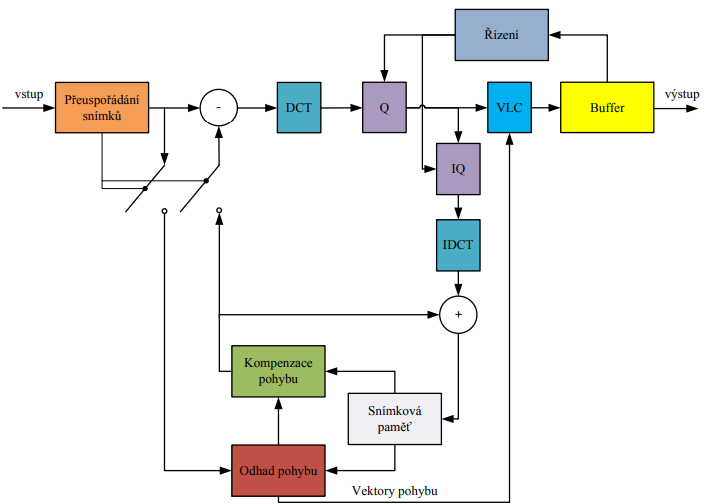
\includegraphics[width=0.7\linewidth]{images/mpeg-koder.png}
\end{figure}
\FloatBarrier

\textbf{Hierarchie:} \vspace{-4mm}
\begin{itemize}
    \item \textbf{Sekvence} – celá videosekvence (celý film)
 \item Skupina snímků (GOP – Group of pictures) – série jednoho nebo více snímků, videosekvence se skládá ze série GOP
jdoucích po sobě, každá GOP začíná snímkem I, délka GOP je dána vzdáleností dvou I snímků, pořadí snímání GOP
se liší od pořadí kódování,
 \item \textbf{Snímek}:
 \begin{itemize}
     \item Snímek I – referenční snímek pro další snímky, kódován principem jako JPEG (první snímek GOP), jsou v něm
všechny obrazové informace,
\item Snímek P – referenční snímek, prediktivně kódován z předchozích referenčního, obsahuje pouze rozdíly oproti
předchozímu snímku, jsou o hodně menší než I snímky
\item Snímek B – není referenční pro další snímky, prediktivně kódován z předchozího i následujícího
\item Snímek D – není referenční, kódují se jako JPEG, ale pouze DC složky
\item Při kódování se standardně používá YCbCr model
 \end{itemize}
 \item \textbf{Slice} – část snímku, minimálně jeden makroblok, maximálně celý snímek
 \item \textbf{Makroblok} – 16x16 pixelů, obsahuje všechny barevné složky obrazu, MPEG-1 vzorkuje makrobloky 4:2:0 YCbCr
 \begin{itemize}
     \item Skládá se z 4x 8x8 px složky Y, 1x 8x8 px složky Cr, 1x 8x8 px složky Cb
\item Kódování makrobloků je INTRA (stejné jako JPEG, rozdílné jen kvantizační tabulky) nebo INTER (kódování rozdílu
aktuálního a referenčního makrobloku, použití u P a B snímků)
 \end{itemize}
\end{itemize}

\begin{figure}[ht]
    \centering
    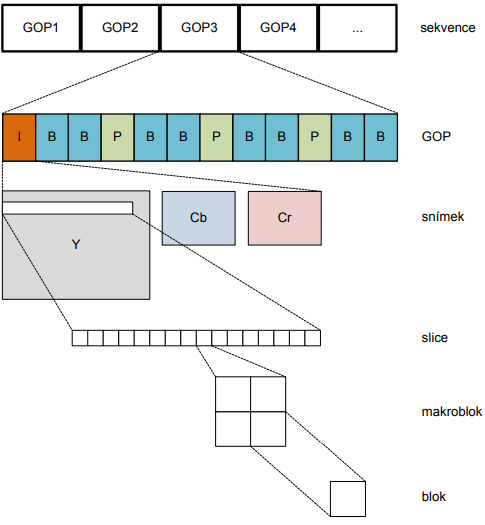
\includegraphics[width=0.5\linewidth]{images/mpeg.png}
\end{figure}
\FloatBarrier

\subsubsection{MPEG-2}
Lepší kvalita obrazu, bitová rychlost 4-100 Mb/s, podpora prokládaného řádkování, kompatibilní s MPEG1, podpora konstantní CBR tak variabilní VBR. \textbf{Využití}: DVD, BlueRay, TV, DVB-T …

\subsubsection{MPEG-4}
\textbf{Kódování objektů videa}
Efektivní komprese progresivního i prokládaného videa.
Podpora: \vspace{-4mm}
\begin{itemize}
    \item kódování statických obrazových dat
    \item efektivního přenosu přes datové sítě 
    \item kódování animovaných objektů 
    \item kódování ve studiové kvalitě.
\end{itemize}

\subsection{H.26x}

Standard MPEG-4 Part 10 / H.264 byl vyvinut společným úsilím organizací ISO (MPEG)
a ITU-T (H.26x) a byl nazván jako AVC (Advanced Video Coding). Princip komprese a
dekomprese vychází ze standardů H.263 a MPEG-2. Základní schéma kodéru vychází z obecného standardu MPEG. Jak je ze schémat patrné, princip kódování i dekódování reflektuje předchozí standardy. Navíc obsahuje deblocking filtr a liší se funkcemi jednotlivých bloků.

\begin{figure}[ht]
    \centering
    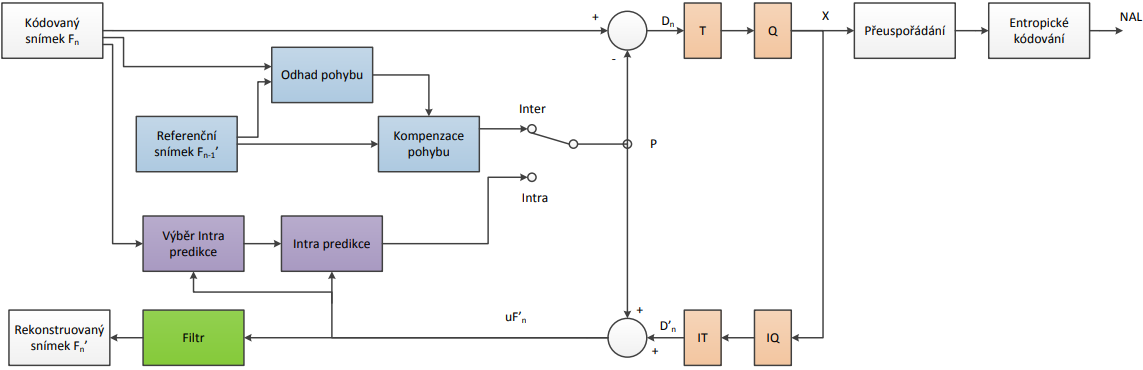
\includegraphics[width=1\linewidth]{images/h264.png}
\end{figure}
\FloatBarrier

\textbf{Základní princip kodéru:}\vspace{-4mm}

Vstupní snímek $F_n$ je rozdělen na \textbf{makrobloky}, kdy každý makroblok je kódován buď v módu \textbf{INTER} nebo \textbf{INTRA}. Pro každý blok makrobloku je na základě rekonstruovaného snímku \textbf{vytvořena predikce P}.

V módu \textbf{INTRA} je predikce P vytvořena ze vzorků právě kódovaného proužku (vzorek již byl kódován, dekódován a rekonstruován).

V módu \textbf{INTER} je predikce P vytvořena pomocí \textbf{pohybové kompenzace} z vybraného jednoho nebo dvou referenčních snímků $F_{n-1}^r$. Referenční snímek může být předešlý nebo budoucí, musí být již zakódovaný, dekódovaný a filtrovaný.

\textbf{Predikce} je následně \textbf{odečtena} od aktuálně kódovaného bloku, čímž vznikne blok $D_n$, který je následně podroben \textbf{transformaci} a \textbf{kvantizaci}. Po těchto úkonech vznikne blok X, který společně s ostatními bloky snímku je \textbf{přeuspořádán} a \textbf{entropicky kódován} a odeslán do vrstvy NAL (vrstva obsahující datové jednotky pro přenos nebo uložení).

Kromě kódování bloků jsou tyto bloky také dekódovány a rekonstruovány pro následnou predikci. Blok X je inverzně kvantován a inverzně transformován tak, že vytvoří rozdílový blok $D'_n$.


\subsection{Metody, které zvyšují účinnost komprese}

a


\section{Video na vyžádání, progresivní stahování, streaming a adaptivní streaming a používané standardy, zabezpečení streamovaného obsahu.}

\subsection{Video na vyžádání}

Technologie umožňující \textbf{on-line ovládání videosekvence z} určité vzdálené \textbf{databáze}. Technologie VoD podporuje všechny služby, které jsou známy z klasického videorekordéru. Dnes součástí mnoha internetových služeb. V rámci sítí využívá protokoly \textbf{RTP}, \textbf{RTSP}. Do VoD řadíme také adaptivní streaming. Klient může sledovat vybrané video a může s ním i vzdáleně manipulovat.

\subsection{Progresivní stahování}

Obsah je nejprve \textbf{stažen a uložen} na lokálním úložišti, \textbf{následně} je \textbf{přehrán}. Využívá http/https přes TCP protokol. U videa umožňuje začít přehrávat dříve, než je celý soubor stažen.

\subsection{Streaming}

Využívá speciální streamovací servery (CDN). Využívá \textbf{RTMP} nebo \textbf{RTSP} protokol. Přenáší se části videa (chunky), které jsou přehrávány v přehrávači -- \textbf{video se neukládá} na lokální disk. Podporuje živé vysílání.

\subsection{Adaptivní streaming}

Umožňuje \textbf{dynamicky měnit kvalitu} videa podle kapacity sítě, procesoru apod. Používá soubor manifest, ve kterém jsou informace o všech částech (chunkách). Adobe HDS (HTTP Dynamic Streaming), \textbf{Apple HLS} (HTTP Live Streaming), Microsoft Smooth Streaming, \textbf{MPEG DASH}.

\subsection{Používané standardy}

\textbf{Real-Time Streaming Protocol (RTSP)} -- Síťový dálkový ovladač. Signalizační protokol pro řízení přenosu dat (např. protokolem RTP). Metody PLAY , PAUSE, RECORD, SETUP, SET\_PARAMETER, GET\_PARAMETER, OPTIONS, REDIRECT, DESCRIBE, TEARDOWN.

\textbf{MPEG DASH}
je standard pro adaptivní streamování videí s proměnlivým datovým tokem, který umožňuje streamovat video obsah na internetu ve vysoké kvalitě. \textbf{Umožňuje}: \vspace{-4mm}

\begin{itemize}
    \item Přepínání mezi streamy různé kvality
\item Vložení reklamy mezi periody
\item Více URL pro stejný obsah v kooperaci s CDN
\item Měření kvality doručeného obsahu
\end{itemize}

\subsubsection{Media Presentation Description (MPD)}
XML dokument popisující multimediální obsah. Pro klienty DASH, získání informací o: \vspace{-4mm}
\begin{itemize}
    \item časování, rozlišení, Zabezpečení
\item dostupnosti  a typu médií,
\item minimální/maximální potřebné šířce pásma,
\item existenci různých alternativ,
\end{itemize}

Popis MPD obsahuje jednu nebo více intervalů (period) daného programu. Každá perioda obsahuje informace o začátku, délku trvání a dále obsahuje jednu nebo více adaptačních množin (AS – adaptation sets). Adaptační množina obsahuje jedno nebo více různě kódovaných médií stejného obsahu (Representation). Každá reprezentace obsahuje informace o daném segmentu.

\textbf{HTTP Live Streaming (HLS)} je protokol pro streamování ohraničených či neohraničených multimediálních dat, možnost přizpůsobení datového toku aktuální propustnosti sítě.

\subsubsection{HLS playlist}
Je přenášen pomocí http(s). Obsahuje segmenty (chunky). První řádek identifikuje formát, další řádek definuje délku každého segmentu, dále následuje popis segmentů. Existence Master Playlistu -- obsahuje různé varianty stejného obsahu (různé kódování, formát, přenosová rychlost apod.)

\subsubsection{HLS segmenty}
Jsou odkazovány z playlistu a mají konkrétní URL. Obsahují informace pro dekódování segmentu. Každý následující segment musí navazovat na segment předchozí. Trvání segmentu je definováno značkou EXTINF.


\subsection{Zabezpečení streamovaného obsahu}

Řeší se prostřednictvím metod správy digitálního obsahu \textbf{DRM} (Digital Rights Management). Řeší ochranu obsahu před jeho neoprávněným šířením. Často využívané standardy -- Google Widevine DRM, Microsoft PlayReady DRM,  Apple FairPlay DRM. Všechna uvedená řešení využívají šifrování pomocí AES 128 bit. \textbf{Funkce} poskytované DRM -- Autentizace, Licencování, Platby, Ochrana soukromí, Sledování porušování práv

